\def\filedate{2009-02-24}\let\thedate\filedate % packages may change \filedate

\documentclass[twoside]{article}
\usepackage{natbib}
\usepackage{chem}
%\usepackage{afterpage}
\usepackage{url}
\usepackage{color}
%\usepackage{multicol}
\usepackage{rotating} % loads graphicx
%\usepackage{longtable}
\usepackage{graphicx}
%\usepackage{eclclass}
%\usepackage{verbatim}

% activate to show "draft" watermark:
%\usepackage{pdfdraftcopy}

\oddsidemargin0mm
\evensidemargin-10mm
\topmargin-10mm
\textheight230mm
\textwidth170mm
\raggedbottom
\parindent0mm
\parskip1.0ex plus0.5ex minus0.5ex
\renewcommand{\arraystretch}{1}
\renewcommand{\topfraction}{0.95}
\renewcommand{\dbltopfraction}{0.95}
\renewcommand{\bottomfraction}{0.95}
\renewcommand{\floatpagefraction}{0.95}
\renewcommand{\dblfloatpagefraction}{0.95}
\renewcommand{\textfraction}{0.01}
\setcounter{topnumber}{3}
\setcounter{bottomnumber}{3}

\newcommand{\todo}[1]{{\uppercase{\bf ((#1))}}}
\newcommand{\egcite}[1]{\citep[e.g.][]{#1}}

\def\nosep{\setlength\parsep{0mm}\setlength\topsep{0mm}\setlength\itemsep{0mm}}

\def\mypageheader{Sander et al.: CAABA/MECCA User Manual}
\markboth{\mypageheader}{\mypageheader}
\pagestyle{myheadings}

% This file was created automatically by xmecca, DO NOT EDIT!
% xmecca was run on 2010-08-26 at 14:15:43 by caaba
\def\meccaversion{\code{2.7b}}
\def\kppversion{\code{2.2.1_rs5}}
\def\wanted{\code{Tr && G && !S && !Cl && !Br && !I && !Hg}}
\def\apn{0}
\def\gasspc{448}
\def\aqspc{0}
\def\allspc{448}
\def\Geqns{246}
\def\Aeqns{0}
\def\Heqns{0}
\def\Jeqns{72}
\def\HETeqns{0}
\def\EQeqns{0}
\def\IEXeqns{0}
\def\Deqns{0}
\def\alleqns{318}
 % \def\meccaversion{...}

\begin{document}

\thispagestyle{empty}

\begin{center}
  
\includegraphics[height=0.3\textheight]{caaba_mecca_logo_print}\\[10mm]
  {\Huge\bf CAABA/MECCA-{\meccaversion} User Manual}\\[10mm]
  {\huge\em \underline{C}hemistry \underline{A}s \underline{A}
    \underline{B}oxmodel \underline{A}pplication /}\\[3mm]
  {\huge\em \underline{M}odule \underline{E}fficiently
    \underline{C}alculating the\\[5mm]
    \underline{C}hemistry of the
    \underline{A}tmosphere}\\[10mm]
  {\huge\bf Rolf Sander, Patrick J\"ockel, Astrid Kerkweg \& Hella
    Riede}\\[15mm]
  \Large
  Air Chemistry Department\\
  Max-Planck Institute of Chemistry\\
  PO Box 3060, 55020 Mainz, Germany\\
  \url{sander@mpch-mainz.mpg.de}\\[10mm]
  {\huge\url{www.mpch-mainz.mpg.de/~sander/messy/mecca/}}
  \vfill
  Date: \thedate
\end{center}

\clearpage

\setlength{\columnsep}{8mm}
\twocolumn\sloppy

\tableofcontents

\begin{figure*}[htb]
  \begin{center}
  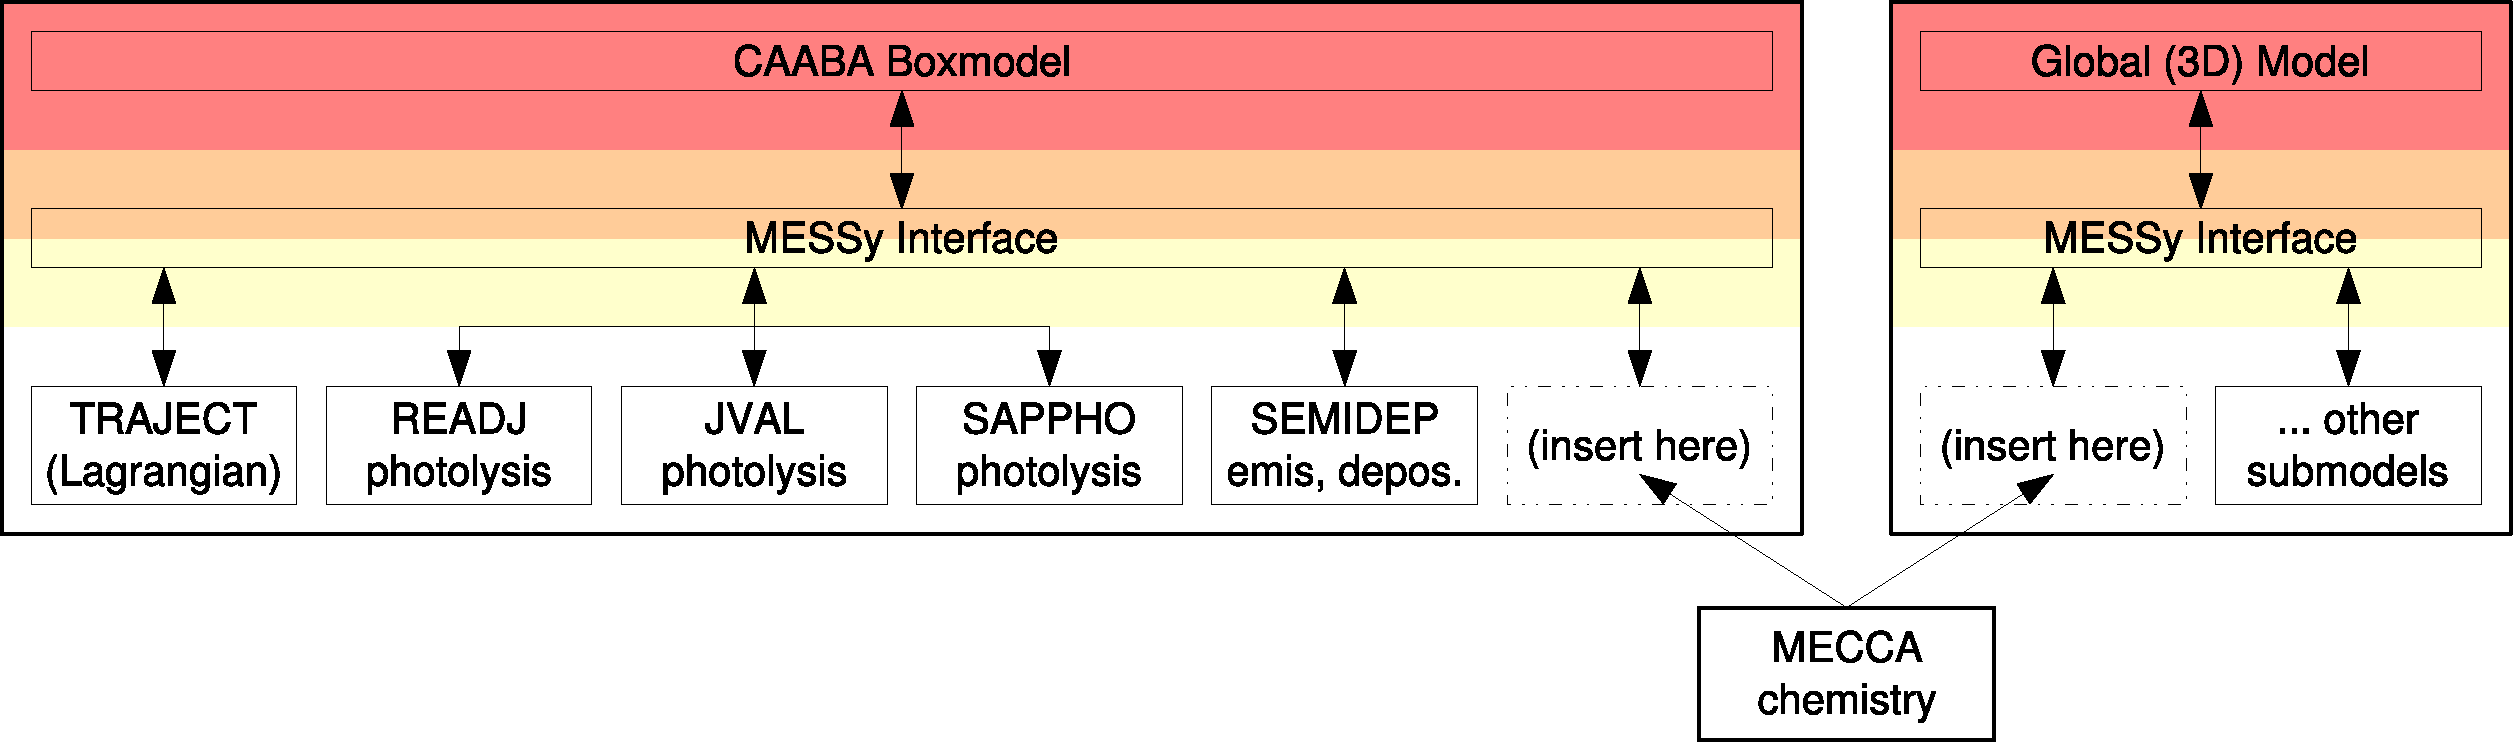
\includegraphics[width=0.9\textwidth]{modular-mecca}
  \end{center}
  \caption{Diagram showing MECCA as part of the CAABA box model or of a
    global model.}
  \label{fig:modular-mecca}
\end{figure*}

\begin{table*}[htb]
  \begin{center}
    \caption{List of CAABA/MECCA Fortran90 files}
    \label{tab:files}
    \begin{tabular}{lp{0.5\textwidth}}
      \hline
      \multicolumn{2}{l}{CAABA box model related files}\\
      \hline
      \verb|caaba.f90|                         & main box model file\\
      \verb|caaba_io.f90|                      & input/output\\
      \verb|caaba_io_netcdf.inc|               & netCDF input/output\\
      \verb|caaba_io_ascii.inc|                & ascii input/output\\
      \verb|caaba_mem.f90|                     & declaration of CAABA variables\\
      \verb|messy_main_control_cb.f90|         & flow control\\
      \verb|messy_jval_box.f90|                & connection of JVAL to CAABA\\
      \verb|messy_mecca_box.f90|               & connection of MECCA to CAABA\\
      \verb|messy_sappho_box.f90|              & connection of SAPPHO to CAABA\\
      \verb|messy_semidep_box.f90|             & simplified emission and
                                                 deposition, including
                                                 connection to CAABA\\
      \verb|messy_traject_box.f90|             & trajectory calculations
                                                 (under construction)\\ 
      % \hline
      % \multicolumn{2}{l}{ECHAM5 related files}\\
      % \hline
      % \verb|messy_mecca_e5.f90|                & interface between ECHAM5 and
      %                                            MECCA subroutines\\
      % \verb|messy_mecca_aero_e5.f90|           & interface between ECHAM5 and
      % MECCA-AERO subroutines\\
      % \verb|messy_mecca_mem_e5.f90|            & declaration and
      %                                            memory for variables\\ 
      % \verb|messy_mecca_idt_e5.inc|            & include file\\
      % \verb|messy_mecca_c2mr_e5.inc|           & include file\\
      % \verb|messy_mecca_mr2c_e5.inc|           & include file\\
      % \verb|messy_mecca_trac_e5.inc|           & include file\\
      % \verb|mecca_t.nml|                       & namelist for tracer
      %                                            initialization\\
      \hline
      \multicolumn{2}{l}{static core files}\\
      \hline
      \verb|messy_main_constants_mem.f90|      & physical constants\\
      \verb|messy_main_blather.f90|            & print utilities\\
      \verb|messy_main_tools.f90|              & auxiliary functions\\
      \verb|messy_main_tools_kp4_compress.f90| & (file exists but is not
                                                 not used with CAABA)\\
      \verb|messy_jval.f90|                    & calculation of J-values\\
      \verb|messy_sappho.f90|                  & simplified and parameterized 
                                                 photolysis rate coefficients\\
      \hline
      \multicolumn{2}{l}{static MECCA core files in the {\tt mecca/smcl/}
        directory}\\
      \hline
      \verb|messy_mecca.f90|                   & MECCA core\\
      \verb|messy_mecca_aero.f90|              & aerosol chemistry\\
      \verb|messy_mecca_khet.f90|              & (file exists but is not
                                                 used with CAABA)\\
      \hline
      \multicolumn{2}{l}{KPP- and {\tt xmecca}-produced files in the {\tt
          mecca/smcl/} directory}\\
      \hline
      \verb|messy_mecca_kpp.f90|               & a wrapper for the KPP files\\
      \verb|messy_mecca_kpp_function.f90|      & ODE function\\
      \verb|messy_mecca_kpp_global.f90|        & global data headers\\
      \verb|messy_mecca_kpp_initialize.f90|    & initialization\\
      \verb|messy_mecca_kpp_integrator.f90|    & numerical integration\\
      \verb|messy_mecca_kpp_jacobian.f90|      & ODE Jacobian\\
      \verb|messy_mecca_kpp_jacobiansp.f90|    & Jacobian sparsity\\
      \verb|messy_mecca_kpp_linearalgebra.f90| & sparse linear algebra\\
      \verb|messy_mecca_kpp_monitor.f90|       & equation info\\
      \verb|messy_mecca_kpp_parameters.f90|    & model parameters\\
      \verb|messy_mecca_kpp_precision.f90|     & arithmetic precision\\
      \verb|messy_mecca_kpp_rates.f90|         & user-defined rate laws\\
      \verb|messy_mecca_kpp_util.f90|          & utility input-output\\
      \hline
      \multicolumn{2}{l}{namelist files}\\
      \hline
      \verb|caaba.nml|                         & CAABA namelist\\
      \verb|jval.nml|                          & JVAL namelist\\
      \verb|mecca.nml|                         & MECCA namelist\\
      \hline
    \end{tabular}
  \end{center}
\end{table*}

\section{Introduction}

MECCA (\underline{M}odule \underline{E}fficiently
\underline{C}alculating the \underline{C}hemistry of the
\underline{A}tmosphere) is an atmospheric chemistry module that contains
a comprehensive chemical mechanism with tropospheric and stratospheric
chemistry of both the gas and the aqueous phase \citep{1666}. For the
numerical integration, MECCA uses the KPP software \citep{1665}.

To apply the MECCA chemistry to an atmospheric scenario, MECCA must be
connected to a base model. As shown in Fig.~\ref{fig:modular-mecca}, the
base model can be a complex, 3-dimensional model \egcite{1851} but it
can also be a simple box model. The connection is established via the
MESSy interface (\url{http://www.messy-interface.org}) developed by
\citet{1664}.

This manual describes how to install and work with MECCA when it is
connected to the box model CAABA (\underline{C}hemistry \underline{A}s
\underline{A} \underline{B}oxmodel \underline{A}pplication). This
combination will be referred to as ``CAABA/MECCA''. The main features of
the CAABA box model are shown in Fig.~\ref{fig:caaba_sketch}. In
addition to MECCA chemistry, CAABA also contains modules for calculating
J-values (JVAL), simplified and parameterized photolysis rates (SAPPHO),
and simplified emission and depostion (SEMIDEP).

\section{Installation}
\label{sec:install}

This section can be skipped if CAABA/MECCA is already installed on your
computer.

CAABA/MECCA has been tested successfully on several UNIX-like operating
systems. The easiest installation is probably on a Linux PC since
several auxiliary programs are already included in a typical Linux
distribution. Installation under ``Windows'' is neither recommended nor
supported. CAABA/MECCA consists of the Fortran90 files listed in
Tab.~\ref{tab:files}. The prerequisites are:
\begin{description}
\item[A Fortran90 compiler (mandatory):] Several compilers have been
  tested successfully: g95 (for Linux), Lahey (for Linux), Intel (for
  Linux), Compaq (Alpha UNIX). Other compilers can be used as well if
  they accept standard Fortran90 code. It should be noted that the g95
  compiler for Linux is free and can be downloaded from
  \url{http://www.g95.org/}.
\item[The Kinetic PreProcessor KPP (mandatory):] This flexible numerical
  integration package by \citet{1665} transforms the chemistry mechanism
  into a set of ordinary differential equations (ODEs) in Fortran90
  syntax. MECCA needs the KPP version that is provided in the
  \verb|mecca/kpp/| directory.
\item[Perl, tcsh, gawk, sed, and make (mandatory):] These UNIX tools are
  standard on Linux systems. Please check that recent versions of them
  are installed. Especially gawk may lead to strange error messages.
  To test gawk, type:\\
  \verb|gawk 'BEGIN {print match("X","[^a-z]")}'|\\
  The result should be ``1''. However, you may get ``0'' as the result
  on your system. Supposedly, this is not a bug in gawk but a feature.
  You can solve the problem by setting the environment variable
  \verb|LC_COLLATE| to ``\verb|C|'':\\
  \verb|export LC_COLLATE=C| $\qquad$ (if you use bash)\\
  \verb|setenv LC_COLLATE C| $\qquad$ (if you use tcsh)\\
  When you try the gawk test again, it should work fine.
\item[La\TeX\ (optional):] If you have La\TeX\ installed on your
  computer, you can print a table (including rate coefficients and
  references) of the currently selected mechanism (see
  Sect.~\ref{sec:latextable} for details).
\item[netCDF library (optional):] The netCDF library is needed to create
  model output in netCDF format. It can be obtained from
  \url{http://www.unidata.ucar.edu/software/netcdf/}. Software for
  manipulating or displaying netCDF data is listed at:
  \url{http://www.unidata.ucar.edu/software/netcdf/software.html}. If
  you don't have the netCDF library, you can still run the model but
  produce only ascii output.
\item[ferret (optional):] The ferret plotting program is needed to plot
  the contents of the netCDF output using the ferret scripts in the
  \verb|jnl/| directory (see Sect.~\ref{sec:ferret} for details).
\end{description}

\begin{figure*}[htb]
  \begin{center}
  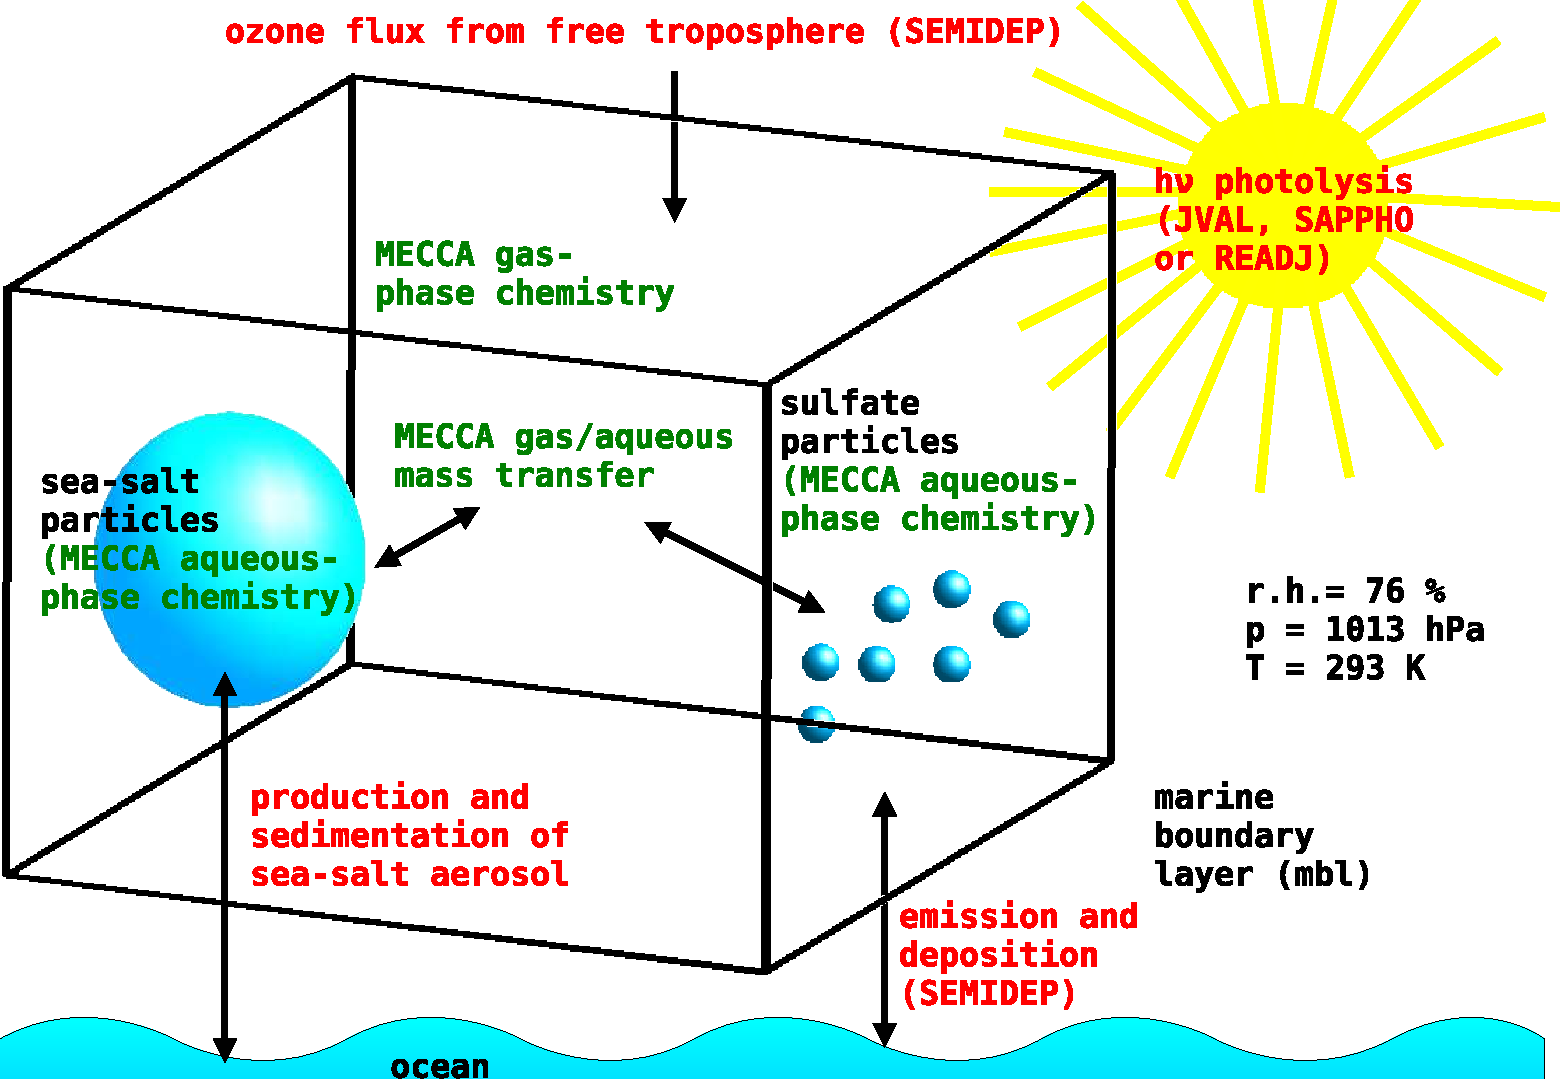
\includegraphics[width=0.9\textwidth]{caaba_sketch}
  \end{center}
  \caption{The CAABA box model}
  \label{fig:caaba_sketch}
\end{figure*}

Once all prerequisites are fulfilled, you can install CAABA/MECCA by
simply unpacking the zip archive:\\[2mm]
{\tt unzip caaba\_\meccaversion.zip}\\[2mm]
Please make sure that the directory structure has not changed during the
unzipping process. Unfortunately, some unzipping programs seem to put
all files into one directory, ignoring the original directory structure.

Next, you have to check that all settings in \verb|Makefile| are
correct. If necessary, edit the file: Choose a Fortran90 compiler
(\verb|COMPILER|), enter its name (\verb|F90|) and the compiler options
(\verb|F90FLAGS|). If you add a new compiler, be sure to activate the
C-preprocessor option. Values for \verb|NETCDF_INCLUDE| and
\verb|NETCDF_LIB| are only needed for the model run when netCDF output
is selected. To activate netCDF output, you also have to edit the
\verb|Makefile|:
\begin{itemize}\nosep
\item Change the variable \verb|OUTPUT| from \verb|ASCII| to
  \verb|NETCDF|.
\item Enter the correct netCDF library information in
  \verb|NETCDF_INCLUDE| and \verb|NETCDF_LIB|.
\end{itemize}

Should there be any problems with the CAABA/MECCA installation, please
check the following:
\begin{itemize}\nosep
\item Confirm that all prerequisites (see above) are fulfilled!
\item Confirm that the perl path in the first line of
  \verb|sfmakedepend| is correct. It should be the same as the output of
  the command:\\
  \verb|which perl|
\item Confirm that the tcsh paths in the first lines of
  \verb|xcaaba| and \verb|xmecca| are correct.
\end{itemize}

\section{Compiling and running the CAABA/MECCA box model with the shell
  script {\tt xcaaba}}
\label{sec:execute}

First, go to the directory of the model code:\\[2mm]
{\tt cd caaba\_\meccaversion}\\[2mm]
Now the tcsh script \verb|xcaaba| guides you through the process of
running the box model. To execute it, type:
\begin{verbatim}
./xcaaba
\end{verbatim}
First, you are asked if you want to create a chemical mechanism with
\verb|xmecca|. If you answer ``y'', you can select a new chemical
mechanism with \verb|xmecca| as described in detail in
Sect.~\ref{sec:xmecca}. However, for the first tests with CAABA/MECCA it
is recommended to answer ``n'' and use the default mechanism, i.e.\
marine gas-phase and aerosol chemistry including halogens. Next, when
asked for an option, choose ``c'' to compile the Fortran90 code. After a
successful compilation, \verb|xcaaba| asks if you want to run the CAABA
boxmodel. After answering ``y'', \verb|xcaaba| lists the active contents
of the \verb|CAABA| and \verb|CTRL| namelists which control the
behaviour of CAABA/MECCA during run-time. The namelists are contained in
the files \verb|caaba.nml| and \verb|mecca.nml|, and editing them allows
fine-tuning of the model run (see Sect.~\ref{sec:nmlfiles}). However,
for the first tests, the defaults can be used as they are. Answer
``Continue?'' with ``y'', and the model run will start. The model day
and the current solar zenith angle (sza) are printed on the screen
during the model run. The default is to integrate 8 days. After the
model run, \verb|xcaaba| asks if you want to save the model output
inside the \verb|output/| directory.

\section{Plotting the model results with the ferret software}
\label{sec:ferret}

If you have chosen netCDF output, you can plot the model results with
the ferret program (\url{http://ferret.wrc.noaa.gov/Ferret/}). Change
into the \verb|jnl| directory, then start the program by typing
``\verb|ferret|''. When ferret has started, you can plot the gas-phase
species of the latest model run with the ferret script \verb|xxxg.jnl|
by typing:
\begin{verbatim}
go xxxg.jnl
\end{verbatim}
Similarly, \verb|xxxa.jnl| can be used to plot aqueous-phase species:
\begin{verbatim}
go xxxa.jnl
\end{verbatim}
The file \verb|xxxa.jnl| accepts several parameters to modify the plots.
The first parameter should be ``\verb|0d|'' for plotting box model
results. The second parameter can be set to ``\verb|mpl|'' or
``\verb|mpm|'' in order to plot either aqueous-phase concentrations
[\unit{mol/L}] or mixing ratios [\unit{mol(aq)/mol(air)}], respectively.
The third parameter defines the aerosol bin. With two aerosol bins,
``\verb|A01|'' refers to sulfate particles, and ``\verb|A02|'' to
sea-salt particles. As an example, type:
\begin{verbatim}
go xxxa.jnl 0d mpl A01
\end{verbatim}
Photolysis rate coefficients can be plotted with \verb|jval.jnl|:
\begin{verbatim}
go jval.jnl
\end{verbatim}
To plot results from previous runs which are saved in the \verb|output/|
directory, edit the file \verb|setmodelrun.jnl| and enter the paths of
the directories in the ``\verb|GO _define_sensi|'' command. To compare
model runs, you can enter two or more ``\verb|GO _define_sensi|''
commands in \verb|setmodelrun.jnl|. To plot the difference between model
runs, activate the line ``\verb|DEFINE SYMBOL diffplot TRUE|'' in
\verb|setmodelrun.jnl|.

\begin{figure*}
  \begin{center}
    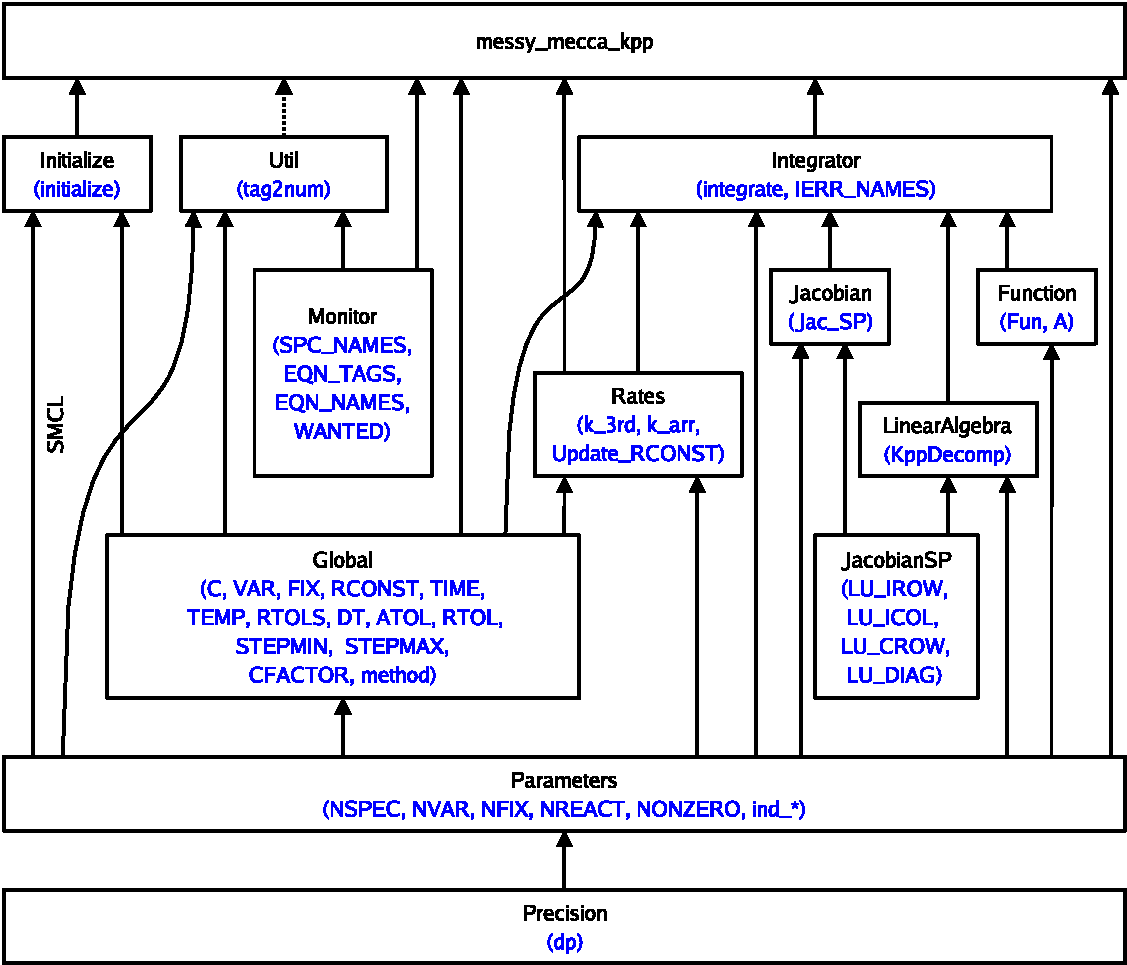
\includegraphics[width=\textwidth]{kpp_use_diagr}
  \end{center}
  \caption{Module structure of KPP-produced Fortran90 files. The arrows
    start at the module which is exporting the variables and subroutines
    shown in blue. They point to the module importing them via the
    Fortran90 USE instruction.}
  \label{fig:kpp_use_diagr}
\end{figure*}

\begin{figure*}
  \begin{center}
    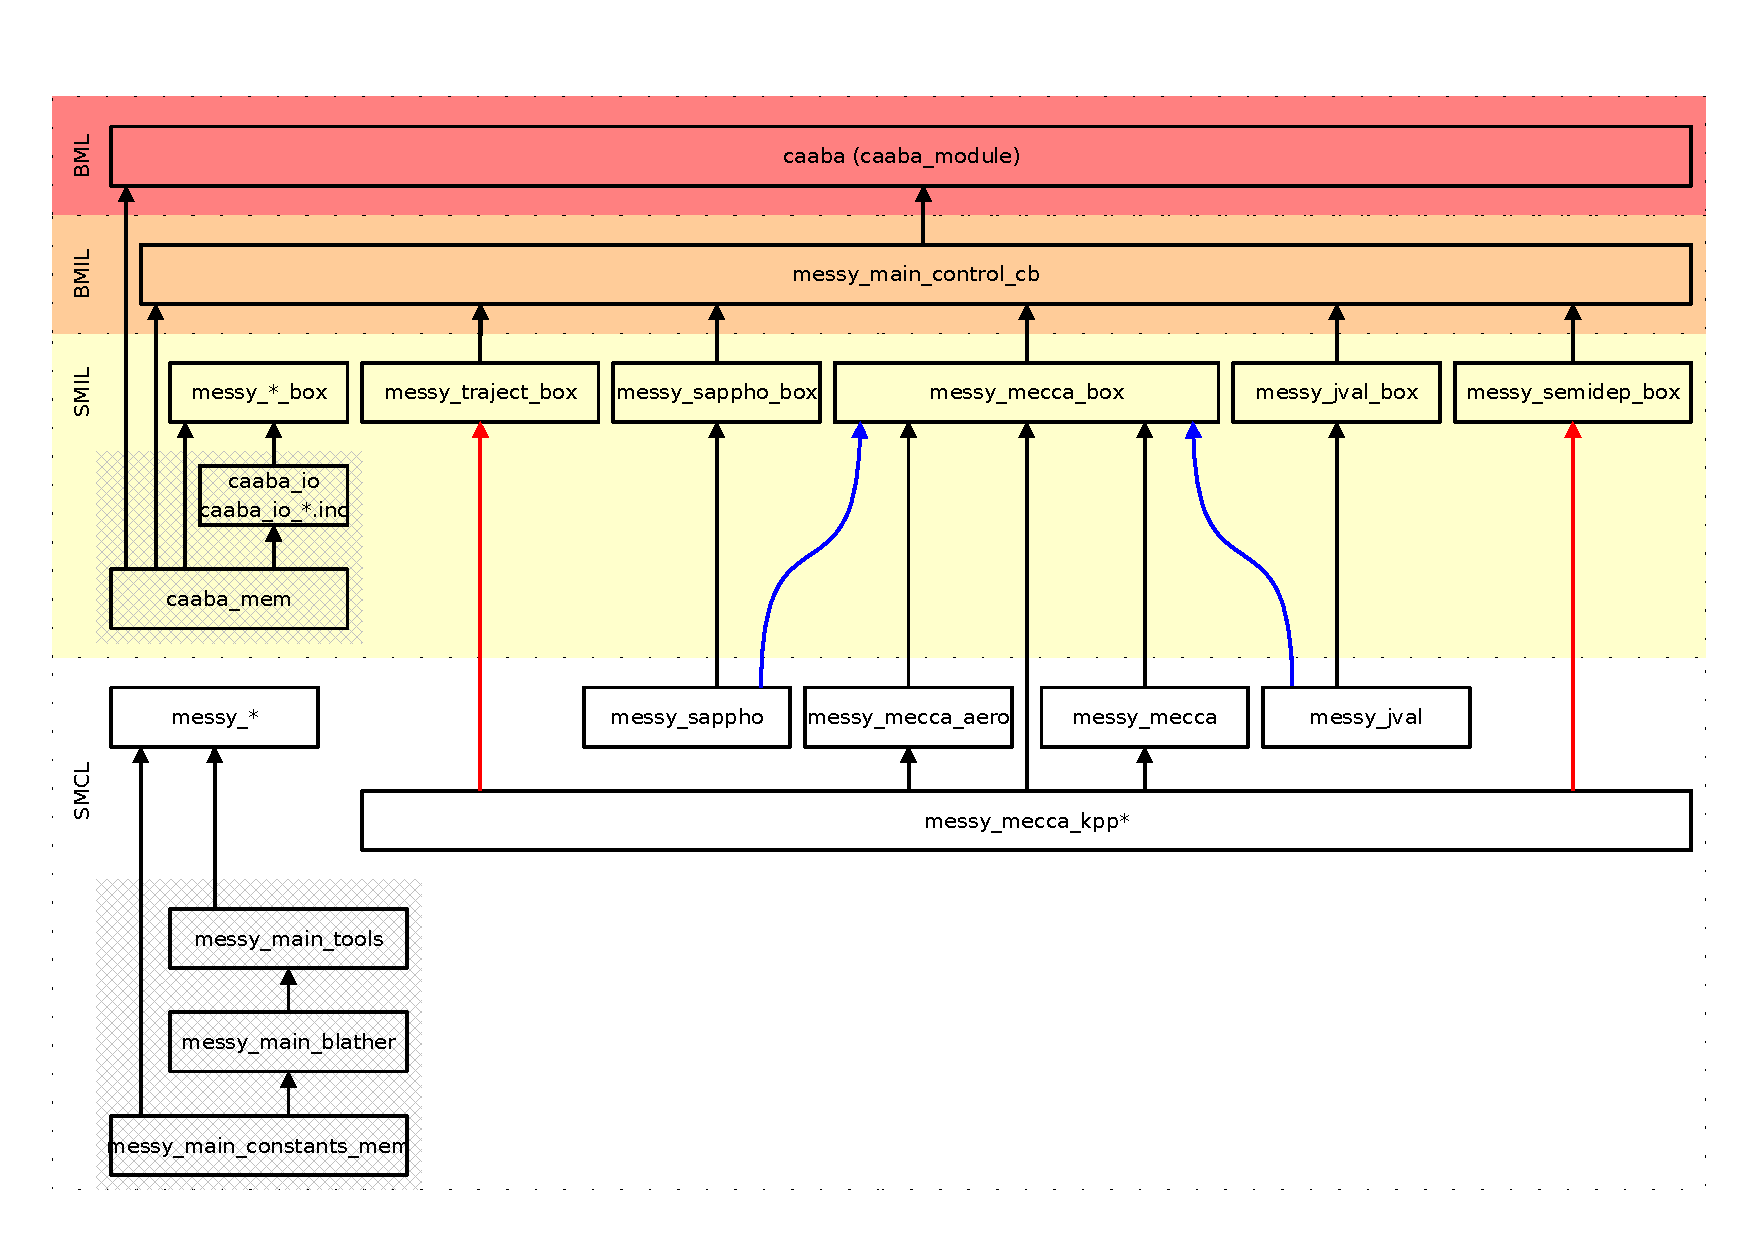
\includegraphics[width=\textwidth]{caaba_use_diagr}
  \end{center}
  \caption{Module structure of MECCA when it is connected to the CAABA
    box model. The box-model related files are in the colored layers
    marked with BML, BMIL, and SMIL. The submodel core layer (SMCL) of
    MECCA is independent of the box model (see \citet{1664} for details
    about the MESSy layers). The arrows start at the module which is
    exporting the variables and subroutines. They point to the module
    importing them via the Fortran90 USE instruction. Here, the box {\tt
      messy\_mecca\_kpp} represents all KPP-generated files. The
    KPP-internal structure is shown in Fig.~\ref{fig:kpp_use_diagr}.}
  \label{fig:caaba_use_diagr}
\end{figure*}

\section{Selecting a chemical mechanism with the shell script {\tt xmecca}}
\label{sec:xmecca}

MECCA contains a very comprehensive set of chemical reactions in both
the gas phase and the aqueous phase. For many applications, using the
complete mechanism will consume too much CPU time. Therefore, the shell
script \verb|xmecca| has been written which allows to create a
custom-made subset of the chemical mechanism interactively. Normally,
\verb|xmecca| is called via \verb|xcaaba|. However, you can also start
it manually:
\begin{verbatim}
cd mecca
./xmecca
\end{verbatim}
\verb|xmecca| will ask several questions, and recommended answers are
given below. If you only press the Return key, you select the default.
\begin{verbatim}
How many aerosol phases? [0...99, default=0]
\end{verbatim}
For a gas-phase only mechanism, type ``0''. For a mechanism with
aqueous-phase chemistry in seasalt and in sulfate particles, type ``2''.
\begin{verbatim}
Modify gas.eqn with a replacement file?
[q/number, default=0]
\end{verbatim}
Answer ``0'' unless you have written your own replacement file. More
information about the replacement feature can be found in the file
\verb|rpl/gas.rpl-example|.
\begin{verbatim}
Choose a selection number or type a boolean
expression [q=quit, default=1]
\end{verbatim}
Now you can choose a subset of chemical reactions. Not all possible
selections have been tested thoroughly. Try one of these:
\begin{description}
\item [Troposphere, Minimum chemistry:] A very small mechanism
\item [Troposphere, Gas, no halogens:] A gas-phase mechanism that
  includes NMHCs
\item [EVAL:] A mechanism that was used for the evaluation of the MECCA
  chemistry in the global model ECHAM5/MESSy.
\item [Minimum MBL chemistry:] A mechanism that contains aqueous-phase
  chemistry and should only be used if the number of aerosol phases is
  $>0$.
\end{description}
For details about the selection, see Sect.~\ref{sec:selectreactions}.
\begin{verbatim}
Add diagnostic tracers to gas.eqn?
[q/0/?, default=0]
\end{verbatim}
When this question shows up, answer ``0''.
\begin{verbatim}
Add diagnostic tracers to all equations?
[y/n/q, default=n]
\end{verbatim}
Answer ``n''.
\begin{verbatim}
Tagging? [y/n/q, default=n]
\end{verbatim}
Tagging is under construction, so please answer ``n''.
\begin{verbatim}
Run KPP?
\end{verbatim}
Answer ``y''.
\begin{verbatim}
Choose an integrator [q=quit,
default=rosenbrock_posdef]:
\end{verbatim}
The default integrator is strongly recommended (see
Sect.\ref{sec:selectintegrator} for details). Next, KPP will create
several Fortran90 files.
\begin{verbatim}
Remove indirect indexing with decomp?
[y/n/q, default=n]
\end{verbatim}
If this question shows up, answer ``n''.
\begin{verbatim}
Create LaTeX listing of selected mechanism?
[y/n/q, default=n]
\end{verbatim}
If you answer ``y'' here, a table of the current reaction mechanism will
be produced. Only the selected reactions will be listed. The table also
contains the rate coefficients and their references, as described in
Sect.~\ref{sec:latextable}.
\begin{verbatim}
Do you want to delete the temporary
xmecca files?
\end{verbatim}
It is okay to delete these temporary files unless you need them for
debugging purposes.

When \verb|xmecca| finishes successfully, the Fortran90 code of your
selected mechanism has been created. The KPP-produced Fortran90 files
(Tab.~\ref{tab:files}) are moved into the \verb|mecca/smcl/| directory
(with lower-case names). An exception is
\verb|messy_mecca_kpp_Model.f90|, which is produced by KPP but not
needed for MECCA. The modular structure of the KPP-produced Fortran90
files is shown in Fig.~\ref{fig:kpp_use_diagr}.

If you need to create a chemical mechanism very often, it is quite
tedious to answer all questions every time. To make this easier, you can
copy the template \verb|batch/example.bat| to a new name (e.g.
\verb|batch/myfile.bat|) and then enter your answers into that file. Now
you can create a new chemical mechanism in batch mode with
\begin{verbatim}
./xmecca myfile
\end{verbatim}

\subsection{Selecting a set of chemical reactions}
\label{sec:selectreactions}

All chemical reactions are marked. Each marker consists of several
labels which contain information about the altitude
(troposphere/stratosphere), the phase where the reaction occurs
(gas/aqueous), its relevant chemical elements, and more. See
Sect.~\ref{sec:markerslabels} for a complete list of labels. To define a
set of chemical reactions, you can either choose a pre-defined selection
by number or enter a boolean expression based on the labels. Boolean
expressions are typed in gawk syntax. The most important operators and
expressions are:\\
\begin{tabular}{l@{ = }l}
\verb|&&| & AND\\
\verb!||! & OR\\
\verb|!|  & NOT\\
\verb|()| & parentheses\\
\verb|1|  & TRUE\\
\verb|0|  & FALSE
\end{tabular}

For example, to select all gas-phase reactions (G) except for those
including halogens (Cl, Br, I), type:

\verb|G && !Cl && !Br && !I|.

It is important to understand the logic behind this selection mechanism.
The expression ``\verb|Cl && Br|'' selects only those reactions that
contain chlorine {\em and} bromine. Similarly, the expression
``\verb|G && Het|'' selects only those reactions that occur in the gas
phase {\em and} and are heterogeneous. However, since no reaction has
both the ``\verb|G|'' {\em and} the ``\verb|Het|'' label, this results
in an empty mechanism. If you want a mechanism that contains both
gas-phase and heterogeneous reactions, you must select all reactions
that contain either the label ``\verb|G|'' {\em or} the label
``\verb|Het|'', i.e.\ you must use the expression ``\verb!G || Het!''.

\subsection{Selecting a numerical integrator}
\label{sec:selectintegrator}

Several numerical integrators are defined in the subdirectory
\verb|mecca/kpp/int/| and can be used with KPP. The default is the
positive definite Rosenbrock solver with automatic time-step control
(\verb|rosenbrock_posdef|). It is very robust and capable of integrating
very stiff sets of equations (e.g.\ chemical mechanisms including both
gas- and aqueous-phase chemistry). Although a Rosenbrock solver with
manual time-step control (\verb|ros2_manual|) is also available, it is
strongly recommended not to use it for stiff sets of equations. If you
choose it, you do so at your own risk!

\section{Modifying CAABA/MECCA}
\label{sec:modifying}

\begin{figure*}[htb]
  \begin{center}
  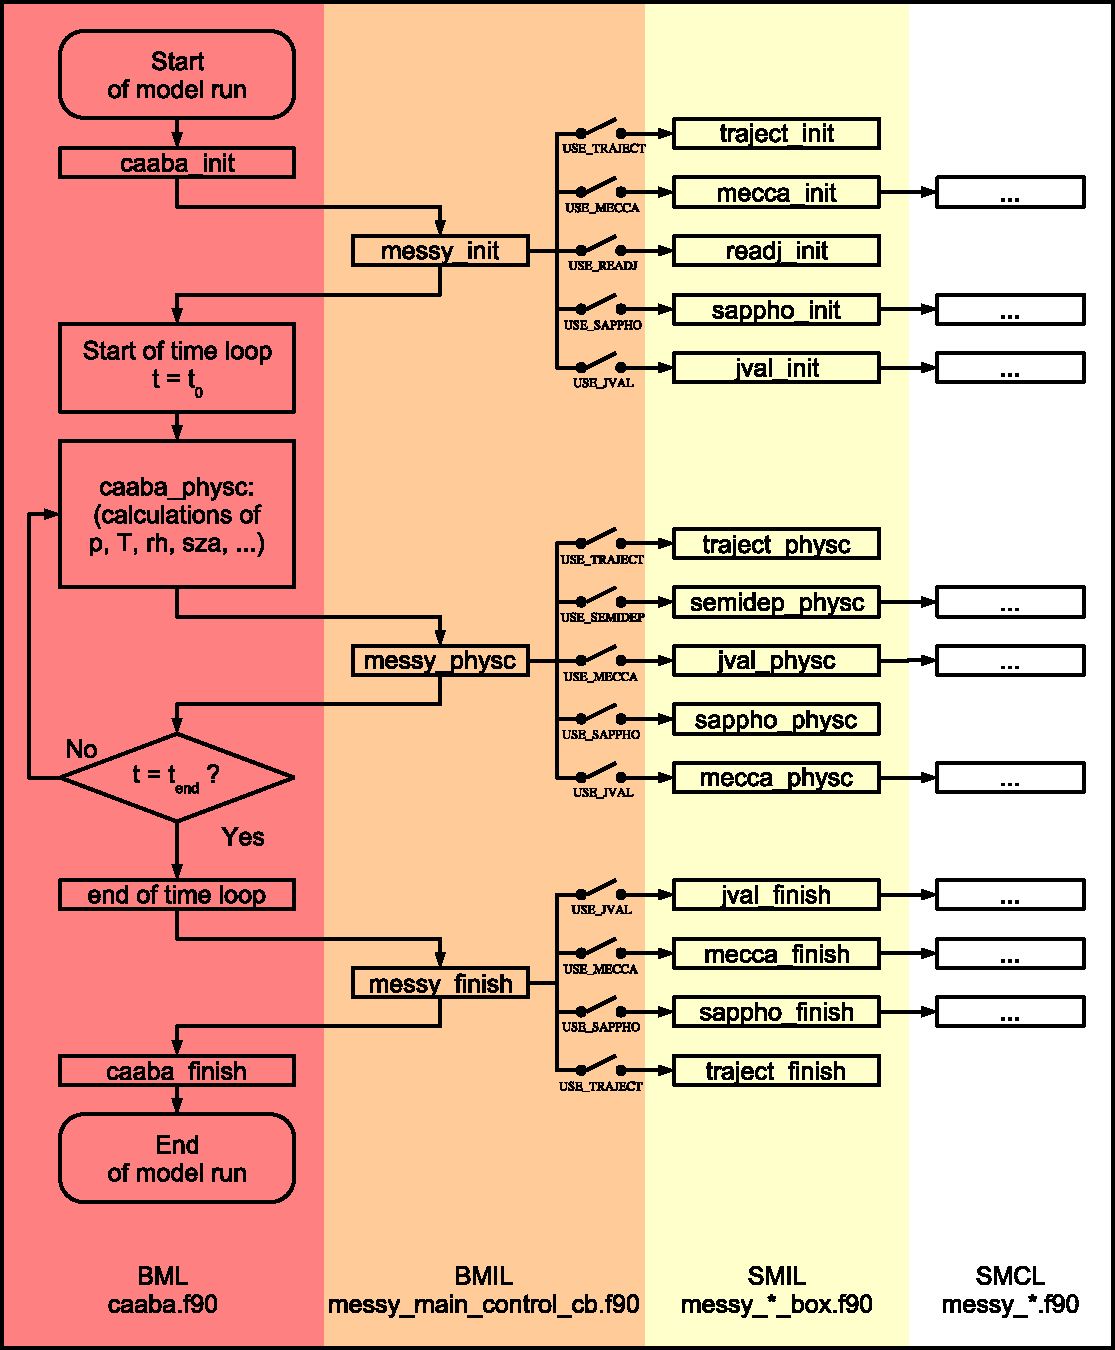
\includegraphics[width=0.9\textwidth]{caaba_flowcontrol}
  \end{center}
  \caption{Flow control of a CAABA box model run}
  \label{fig:caaba_flowcontrol}
\end{figure*}

The flow control of a CAABA/MECCA model simulation is shown in
Fig:~\ref{fig:caaba_flowcontrol}.

The CAABA/MECCA model simulation can be modified by changing the
namelist files (\verb|*.nml|), the species files (\verb|*.spc|), the
equation files (\verb|*.eqn|) and the Fortran90 files (\verb|*.f90|).

\subsection{The namelist files {\tt caaba.nml} and {\tt mecca.nml}}
\label{sec:nmlfiles}

The file \verb|caaba.nml| contains the namelist \verb|&CAABA|. Here
individual parts of the CAABA model (the so-called ``MESSy submodels'')
can be switched on or off. It is important that the following switches
are set to ``T'' (=true):
\begin{verbatim}
USE_MECCA   = T
USE_SAPPHO  = T
USE_SEMIDEP = T
\end{verbatim}
To use the photolysis rate coefficients from SAPPHO in MECCA, set:
\begin{verbatim}
photrat_channel = 'sappho'
\end{verbatim}
Alternatively, you can switch on the JVAL submodel with
\verb|USE_JVAL = T| and then select \verb|photrat_channel = 'jval'|. It
is fine to switch on both the JVAL and the SAPPHO submodel, which can be
useful for a comparison. However, only the values selected by
\verb|photrat_channel| are used for the MECCA chemistry.

You can define the model start, runtime, and time step. e.g.:
\begin{verbatim}
startday    = 90.
ext_runtime = '10 days'
time_step   = '15 minutes'
\end{verbatim}
If you don't set these, the default is a model start on Julian day 80, a
model run duration of 8 days, and an output time step of 20 minutes.

The file \verb|mecca.nml| contains the namelists \verb|&CTRL_KPP| and
\verb|&CTRL| (the namelist \verb|&CPL| is not used in connection with
CAABA). \verb|&CTRL_KPP| is used for fine-tuning the numerical
integration. The default selection \verb|icntrl(3) = 2| should normally
be suitable.

\subsection{The species files {\tt gas.spc} and {\tt aqueous.spc}}
\label{sec:spcfiles}

The files \verb|*.spc| declare chemical species for KPP. All species
that may occur in an equation must be declared here. Additional dummy
species may also be declared here.

Gas-phase species are declared in \verb|gas.spc|. Examples for gas-phase
species are \verb|O2|, \verb|O1D|, and \verb|NO2|. The names of lumped
species start with ``\verb|l_|''.

MECCA also includes aqueous species which are declared in
\verb|aqueous.spc|. The names of cations end with ``\verb|p|'' for plus.
The names of single-charge anions end with ``\verb|m|'' for minus.
Doubly-charged anions end with ``\verb|mm|''. Examples for aqueous
species are \verb|H2O2|, \verb|Hp|, \verb|NO3m|, and \verb|SO4mm|.

All aqueous-phase species have the suffix ``\verb|_a##|'', which is a
placeholder for the aerosol phase number. \verb|xmecca| replaces it by
either ``\verb|_a01|'' (accumulation soluble) or ``\verb|_a02|'' (coarse
soluble). This allows separate chemistry calculations for aerosol
particles of different size and composition.

All species are defined here with \verb|#DEFVAR|, i.e.\ KPP considers
them as prognostic variables. To treat a species as a constant (e.g.\ 
\chem{CO_2}), it can be added to the \verb|#SETFIX| command in the file
\verb|messy_mecca_kpp.kpp|.

\subsection{The equation files {\tt gas.eqn} and {\tt aqueous.eqn}}
\label{sec:eqnfiles}

The equation files \verb|*.eqn| define the chemical reaction mechanism
for KPP. Each reaction occupies one line in this file. An example is:

\begin{verbatim}
<G1000> O2 + O1D = O3P + O2 : {%StTrG}
   3.3E-11*EXP(55./temp); {&1945}
\end{verbatim}

The line starts with the reaction number, which is enclosed in angle
brackets ``\verb|<...>|'' (see Sect.~\ref{sec:rxnnumbers}). The second
part (up to the colon) defines the reaction, and the third part (between
the colon and the semicolon) defines the rate coefficient. The lines may
also contain comments. Comments in equation files are either enclosed in
curly braces, or the comment line starts with \verb|//|. When using
\verb|xmecca|, some comments have a special meaning. Comments starting
with the percent symbol ``\verb|{%...}|''
  are markers (see Sect.~\ref{sec:markerslabels}). Comments starting
  with the ampersand ``\verb|{&...}|'', the ``at''-symbol
  ``\verb|{@...}|'', or the dollar ``\verb|{$...}|'' are used to store
  information for the listing of reactions, as explained in
  Sect.~\ref{sec:latextable}.

If the definition of a rate coefficient is very complex, it can be
stored in a Fortran90 variable and the variable is put into the
\verb|gas.eqn| file. For example, the rate of the self reaction of
\chem{HO_2} is quite complex since it depends on humidity. It is
predefined and the reaction line can be simplified to:
\begin{verbatim}
HO2 + HO2 = H2O2 : k_HO2_HO2;
\end{verbatim}
The declaration and definition of \verb|k_HO2_HO2| are also in the
\verb|gas.eqn| file. They can be found in the so-called KPP ``inline
types'' \verb|F90_GLOBAL| and \verb|F90_RCONST|, e.g.:
\begin{verbatim}
#INLINE F90_GLOBAL
  REAL :: k_HO2_HO2
#ENDINLINE

#INLINE F90_RCONST
  k_HO2_HO2 = (1.5E-12*EXP(19./temp)+ &
              1.7E-33*EXP(1000./temp)*cair)* &
              (1.+1.4E-21* &
              EXP(2200./temp)*C(KPP_H2O))
#ENDINLINE
\end{verbatim}

Another method to add reaction rates with complex dependencies are
Fortran90 functions. This is done for example for the oxidation of
\chem{S(IV)} by \chem{H_2O_2} (\verb|k_SIV_H2O2|). A function call is
given as the rate in the \verb|*.eqn| file. These functions are defined
with the ``inline type'' \verb|F90_RATES|:
\begin{verbatim}
#INLINE F90_RATES
  ELEMENTAL REAL(dp) FUNCTION k_SIV_H2O2 &
    (k_298,tdep,cHp,temp)
    ...
  END FUNCTION k_SIV_H2O2
#ENDINLINE
\end{verbatim}

\subsubsection{Reaction numbers}
\label{sec:rxnnumbers}

Each reaction in an equation file has a unique reaction ``number''
(number is not quite correct, since letters are included as well), which
is enclosed in angle brackets, e.g.: ``\verb|<G1000>|''. The reaction
number starts with one or more upper case letters denoting the type of
reaction. The following types exist:

\begin{tabular}{lp{0.8\columnwidth}}
  A   & aqueous-phase reactions\\
  H   & Henry's law (dissolution and evaporation)\\
  EQ  & equilibria in the aqueous phase (forward and backward reactions of
  acid/base and other equilibria)\\
  G   & gas-phase reactions\\
  J   & J-values of photolysis reactions\\
  HET & heterogeneous reactions (e.g.\ on polar stratospheric clouds)
\end{tabular}

The type is followed by a sequence of 3 or 4 digits. The first digit is
the number of the main element of the reaction. The following numbers
are used:

\begin{tabular}{lll}
  1) & \chem{O}  & Oxygen   \\
  2) & \chem{H}  & Hydrogen \\
  3) & \chem{N}  & Nitrogen \\
  4) & \chem{C}  & Carbon   \\
  5) & \chem{F}  & Fluorine \\
  6) & \chem{Cl} & Chlorine \\
  7) & \chem{Br} & Bromine  \\
  8) & \chem{I}  & Iodine   \\
  9) & \chem{S}  & Sulfur   \\
 10) & \chem{Hg} & Mercury  \\
\end{tabular}

Out of those elements that occur in a reaction, the one with the highest
number is called the main element. Accordingly, the second digit is
determined by the element with the second highest number (or set to zero
if there is no second element in the reaction). There is one exception
in this numbering scheme: For the carbon group, the second digit is the
number of C atoms in the largest organic molecule.

The following digits have no special meaning. If a reaction branches
into several pathways, a suffix ``a'', ``b'', ``c'', \dots\ is added.

\subsubsection{Markers and labels}
\label{sec:markerslabels}

Each reaction must contain a marker. A marker contains several labels.
The syntax is ``\verb|{%...}|'' where the dots represent the
  labels. Labels are used to select specific reactions, as described
  above (Sect.~\ref{sec:selectreactions}). The labels are placed in the
  marker without separators. The following labels are available and
  should appear in this order:
\begin{enumerate}
\item altitudes at which the reaction occurs (mandatory, include at
  least one)\\
  \begin{tabular}{l@{ = }p{0.7\columnwidth}}
  \verb|St|   & Reactions relevant in the stratosphere\\
  \verb|Tr|   & Reactions relevant in the troposphere
  \end{tabular}
\item phase (mandatory, include exactly one)\\
  \begin{tabular}{l@{ = }p{0.7\columnwidth}}
    \verb|Aa##| & Aqueous, aerosol (\verb|##| is a placeholder for the
    2-digit aerosol phase number)\\
    \verb|G|    & Gas phase reactions\\
    \verb|Het|  & heterogeneous reactions (e.g. on polar stratospheric
                  clouds)\\ 
  \end{tabular}
\item elements (include all elements that occur in the reaction, except
  for H and O)\\
  \begin{tabular}{l@{ = }p{0.7\columnwidth}}
  \verb|N|    & Nitrogen\\
  \verb|C|    & Carbon with $>$ 1 C atom (only used for C,N,O species but
                not for halogenated or sulfur-containing organics)\\
  \verb|F|    & Fluorine\\
  \verb|Cl|   & Chlorine\\
  \verb|Br|   & Bromine\\
  \verb|I|    & Iodine\\
  \verb|S|    & Sulfur\\
  \verb|Hg|   & Mercury
  \end{tabular}
\item other\\
  \begin{tabular}{l@{ = }p{0.7\columnwidth}}
  \verb|J|    & Photolysis reactions\\
  \verb|Mbl|  & Minimum reaction mechanism for MBL chemistry\\
  \verb|Sc|   & Scavenging chemistry mechanism\\
  \verb|Scm|  & Scavenging chemistry mechanism, minimum selection
  \end{tabular}
\end{enumerate}

See Sect.~\ref{sec:newlabel} for a description how to add new labels to
\verb|xmecca|.

\subsubsection{Creating a table of the chemical mechanism}
\label{sec:latextable}

To ensure that the documentation of the chemical mechanism is always up
to date, the necessary information is contained inside the species and
equation files. The gawk scripts \verb|spc2tex.awk| and
\verb|eqn2tex.awk| convert information from the selected reactions into
a La\TeX\ table. Bib\TeX\ citations are included in comments starting
with an ampersand ``\verb|{&...}|''. If there is a second ampersand
``\verb|{&&...}|'', additional information about reactions can be found
in \verb|meccanism.tex| as a footnote to the tables. Comments starting
with the at symbol ``\verb|{@...}|'' or the dollar ``\verb|{$...}|'' can
be used to put La\TeX\ commands directly into the \verb|*.eqn| files.
\verb|eqn2tex.awk| produces several \verb|*.tex| files which are
included into \verb|meccanism.tex|.

Creating the document only works if you have the programs \verb|latex|,
\verb|bibtex|, \verb|dvips|, and \verb|gv| installed on your system. If
you want to use different programs (e.g. pdf\LaTeX\ instead of \LaTeX\ 
or a postscript viewer other than \verb|gv|) you can enter the
appropriate commands into \verb|xmecca|.

\subsection{Fortran90 files}
\label{sec:f90files}

The CAABA/MECCA simulations can be modified by changing the Fortran90
files. The modular structure of the Fortran90 files is shown in
Fig.~\ref{fig:caaba_use_diagr}. Most of the files need only be changed
by model developers. Those that are also interesting for model users,
are briefly explained below.

\subsubsection{{\tt caaba.f90}}

This file contains the main Fortran90 code (``\verb|PROGRAM caaba|'').
Here, the values of temperature (\verb|temp|), pressure (\verb|press|),
relative humidity (\verb|relhum|), and the height of the boundary layer
(\verb|zmbl|) can be defined.

\subsubsection{{\tt caaba\_mem.f90}}

This file contains variable declarations which are needed by several
CAABA files.

\subsubsection{{\tt messy\_main\_control\_cb.f90}}

Flow control. Editing this file is only necessary when a new submodel is
added.

\subsubsection{{\tt messy\_jval\_box.f90}}

This file contains the connection of JVAL to CAABA.

\subsubsection{{\tt messy\_jval.f90}}

This file contains the calculation of J-values.

\subsubsection{{\tt messy\_mecca\_box.f90}}

The chemical composition of seawater is defined in
\verb|SUBROUTINE mecca_init|. Aerosol properties (radius, liquid water
content (LWC), and their chemical composition) are defined in
\verb|SUBROUTINE define_aerosol|. Initial mixing ratios of chemical
species are defined in \verb|SUBROUTINE x0|.

\subsubsection{{\tt messy\_sappho\_box.f90}}

This file contains the connection of SAPPHO to CAABA.

\subsubsection{{\tt messy\_sappho.f90}}

Simplified parameterized photolysis rate coefficients are defined here.

\subsubsection{{\tt messy\_semidep\_box.f90}}

Simplified emission fluxes and deposition velocities are defined here.

\subsubsection{{\tt messy\_mecca\_aero.f90}}

Several variables needed to calculate rate coefficients are defined in
\verb|messy_mecca_aero.f90|. The accommodation coefficients
(\verb|alpha|) and the mean velocity (\verb|vmean|) are used for the
calculation of the mass transfer coefficients (\verb|ykmt|). Together
with the inverse dimensionless Henry's law coefficients (\verb|yhenry|),
they are needed to calculate equilibria between the gas and the aqueous
phase. Heterogeneous reactions are described with the forward
(\verb|k_exf|) and backward (\verb|k_exb|) rate coefficients. The
variable \verb|xaer| is set to 1 or 0 to switch aqueous-phase chemistry
on or off, respectively. The factor \verb|cvfac| converts the
aqueous-phase unit \unit{mol/L} (refering to the volume of the liquid)
to the gas-phase unit \unit{molecules/cm^3} (referring to the gas-phase
volume).

\subsection{How to expand the chemical mechanism}

This section contains brief descriptions for experienced model
developers explaining where to make changes to the code for certain
model expansions.

\subsubsection{Adding a new gas-phase species}

\begin{itemize}\nosep
\item \verb|gas.spc|:\\
  Add the new species, its elemental composition,
  the name in La\TeX\ syntax, and a comment, e.g.:\\
  \verb|C4H10 = 4C + 10H ; {@C_4H_<10>} {n-butane}|\\
  Note that curly brackets needed by La\TeX\ must be entered as angle
  brackets.
\end{itemize}

\begin{itemize}\nosep
\item \verb|jnl/xxxg.jnl|:\\
  Add one line per new species. Check if the new species is part of an
  existing familiy, e.g.\ add new reactive bromine species to
  \verb|Brx|.
\end{itemize}

\begin{itemize}\nosep
\item \verb|jnl/tools/_kppvarg.jnl|:\\
  Add one line per new species.
\end{itemize}

\subsubsection{Adding a new aqueous-phase species}

\begin{itemize}\nosep
\item \verb|aqueous.spc|:\\
  Add the new species, the name in La\TeX\ syntax, and a comment,
  e.g.:\\
  \verb|SO4mm_a## = IGNORE; {@SO_4^<2->\aq} {sulfate}|\\
  The suffix \verb|_a##| is mandatory. The elemental composition is
  currently ignored. Note that curly brackets needed by La\TeX\ must be
  entered as angle brackets.
\end{itemize}

\begin{itemize}\nosep
\item \verb|jnl/xxxa.jnl|:\\
  Add one line per new species. 
\end{itemize}

\begin{itemize}\nosep
\item \verb|jnl/_families_a.jnl|:\\
  Check if the new species is part of an existing familiy, e.g.\ add new
  bromine species to \verb|Brtot|.
\end{itemize}

\begin{itemize}\nosep
\item \verb|jnl/tools/_kppvara.jnl|:\\
  Add one line per new species.
\end{itemize}

\subsubsection{Adding a new gas-phase reaction}
\label{sec:addgprxn}

First, choose an appropriate reaction number. To avoid that several
developers assign the same number to different new reactions, it is
strongly recommended that a preliminary reaction number is used
initially. This can be done by adding the developer's initials as a
suffix, e.g.\ John Doe would use \verb|G0001JD|, \verb|G0002JD|,
\verb|G0003JD|, and so on. When the new code is merged with other
development branches, the final reaction numbers will be assigned.

\begin{itemize}\nosep
\item \verb|gas.eqn|:\\
  Add one line per new reaction.
\end{itemize}

\begin{itemize}\nosep
\item \verb|latex/meccanism.tex|:\\
  If necessary, add a footnote about the new reaction here.
\end{itemize}

\begin{itemize}\nosep
\item \verb|jnl/rates.jnl|:\\
  Add one line per new reaction.
\end{itemize}

\subsubsection{Adding a new gas-phase photolysis reaction}

First, choose an appropriate reaction number, as explained in
Sect.~\ref{sec:addgprxn}.

\begin{itemize}\nosep
\item \verb|gas.eqn|:\\
  Add one line per new reaction. Check that the necessary photolysis
  rate coefficient is provided by SAPPHO, READJ, and/or JVAL.
\end{itemize}

\begin{itemize}\nosep
\item \verb|latex/meccanism.tex|:\\
  If necessary, add a footnote about the new reaction here.
\end{itemize}

\begin{itemize}\nosep
\item \verb|jnl/rates.jnl|:\\
  Add one line per new reaction.
\end{itemize}

\subsubsection{Adding a new aqueous-phase reaction}

First, choose an appropriate reaction number, as explained in
Sect.~\ref{sec:addgprxn}.

\begin{itemize}\nosep
\item \verb|aqueous.eqn|:\\
  Add one line per new reaction.
\end{itemize}

\begin{itemize}\nosep
\item \verb|latex/meccanism.tex|:\\
  If necessary, add a footnote about the new reaction here.
\end{itemize}

\begin{itemize}\nosep
\item \verb|jnl/rates.jnl|:\\
  Add one line per new reaction.
\end{itemize}

\subsubsection{Adding a new Henry's law equilibrium}

First, choose an appropriate reaction number, as explained in
Sect.~\ref{sec:addgprxn}.

\begin{itemize}\nosep
\item \verb|aqueous.eqn|:\\
  Add two lines per new equilibrium, one for the forward and one for the
  backward reaction.
\end{itemize}

\begin{itemize}\nosep
\item \verb|messy_mecca_aero.f90|:\\
  Add calculation of \verb|vmean|, \verb|alpha|, and \verb|zhenry| which
  is needed for \verb|k_exf| and \verb|k_exb|.
\end{itemize}

\begin{itemize}\nosep
\item \verb|latex/meccanism.tex|:\\
  If necessary, add a footnote about the new equilibrium here.
\end{itemize}

\begin{itemize}\nosep
\item \verb|jnl/rates.jnl|:\\
  Add two lines per new equilibrium, one to define the net rate and one
  to plot it.
\end{itemize}

\begin{itemize}\nosep
\item \verb|jnl/tools/_kppvarrates.jnl|:\\
  Add one line per new equilibrium.
\end{itemize}

\subsubsection{Adding a new acid-base equilibrium}

First, choose an appropriate reaction number, as explained in
Sect.~\ref{sec:addgprxn}.

\begin{itemize}\nosep
\item \verb|aqueous.eqn|:\\
  Add two lines per new equilibrium, one for the forward and one for the
  backward reaction.
\end{itemize}

\begin{itemize}\nosep
\item \verb|latex/meccanism.tex|:\\
  If necessary, add a footnote about the new equilibrium here.
\end{itemize}

\begin{itemize}\nosep
\item \verb|jnl/rates.jnl|:\\
  Add two lines per new equilibrium, one to define the net rate and one
  to plot it.
\end{itemize}

\begin{itemize}\nosep
\item \verb|jnl/tools/_kppvarrates.jnl|:\\
  Add one line per new equilibrium.
\end{itemize}

\subsubsection{Adding a new label}
\label{sec:newlabel}

First, choose a name for the new label. The name must start with an
upper case letter and can be followed by one or more lower case letters
or numbers. Element symbols must not be used because they are reserved
for reactions of that element. For example, since S is sulfur, the
symbol S could not be used for the stratosphere. To avoid that several
developers introduce new labels with the same name for different
purposes, it is strongly recommended that a preliminary label is used
initially. This can be done by adding the developer's initials as a
prefix, e.g.\ John Doe would use \verb|Jd1|, \verb|Jd2|, \verb|Jd3|, and
so on. When the new code is merged with other development branches, a
final label name can be assigned.

\begin{itemize}\nosep
\item \verb|xmecca|:\\
  In the generation of \verb|awkfile1|, add another \verb|locate|
  function, and print the new label to the logfile.
\end{itemize}

\subsubsection{Adding a new emission}

\begin{itemize}\nosep
\item \verb|messy_mecca_semidep.f90|:\\
  Add one line to \verb|emission_default| (or one of the other
  \verb|emission_*| subroutines).
\end{itemize}

\subsubsection{Adding a new deposition}

\begin{itemize}\nosep
\item \verb|messy_mecca_semidep.f90|:\\
  Add one line to \verb|drydep|.
\end{itemize}

\subsection{How to add a new MESSy submodel}

\begin{itemize}
\item Choose a name (up to 7 alphanumerical characters, starting with a
  letter). Here, ``\verb|xyz|'' is used as an example.
\item \verb|caaba_mem.f90|:\\
  \verb|LOGICAL :: USE_XYZ = .FALSE.|
\item \verb|messy_xyz.f90|:\\
  Put all generic subroutines here, i.e.\ all subroutines that are used
  for the CAABA boxmodel as well as for a global model.
\item \verb|messy_xyz_box.f90|:\\
  Put CAABA-specific code here. Generic code is not included directly
  here. Instead, the generic subroutines in \verb|messy_xyz.f90| are
  called from here. This file contains up to four subroutines:
  \begin{itemize}
  \item If the submodel needs an initialization, put subroutine
    \verb|xyz_init| here.
  \item If the submodel performs calculations during the time loop, put
    subroutine \verb|xyz_physc| here.
  \item If the submodel prints results, put subroutine \verb|xyz_result|
    here.
  \item If the submodel needs to close any open files at the end of the
    model run, put subroutine \verb|xyz_finish| here.
  \end{itemize}
\item \verb|messy_main_control_cb.f90|:
  \begin{itemize}
  \item Add ``\verb|USE_XYZ|'' to ``\verb|USE caaba_mem|''
  \item If subroutine \verb|xyz_init| exists, add:\\
    \verb|USE messy_xyz_box, ONLY: xyz_init|\\
    \verb|IF (USE_XYZ) CALL xyz_init|\\
    to subroutine \verb|messy_init|.
  \item If subroutine \verb|xyz_physc| exists, add:\\
    \verb|USE messy_xyz_box, ONLY: xyz_physc|\\
    \verb|IF (USE_XYZ) CALL xyz_physc|\\
    to subroutine \verb|messy_physc|.
  \item If subroutine \verb|xyz_result| exists, add:\\
    \verb|USE messy_xyz_box, ONLY: xyz_result|\\
    \verb|IF (USE_XYZ) CALL xyz_result|\\
    to subroutine \verb|messy_result|.
  \item If subroutine \verb|xyz_finish| exists, add:\\
    \verb|USE messy_xyz_box, ONLY: xyz_finish|\\
    \verb|IF (USE_XYZ) CALL xyz_finish|\\
    to subroutine \verb|messy_finish|.
  \end{itemize}
\item \verb|caaba.f90|:\\
  Edit subroutine \verb|caaba_read_nml|:
  \begin{itemize}
  \item Add ``\verb|USE_XYZ|'' to ``\verb|USE caaba_mem|''.
  \item Add ``\verb|USE_XYZ|'' to namelist \verb|/CAABA/|.
  \item Print value of \verb|USE_XYZ| (see ``selected MESSy submodels'')
  \item If applicable, perform consistency checks for interaction of new
    submodel with other submodels.
  \end{itemize}
\item \verb|nml/default/caaba.nml|:\\
  Add sensible default values for \verb|USE_XYZ| and possibly other
  options.
\item \verb|manual/caaba_mecca_manual.tex|:\\
  Mention new submodel in this user manual (Sect.~\ref{sec:f90files},
  Tab.~\ref{tab:files}, and Fig.~\ref{fig:caaba_flowcontrol}).
\end{itemize}

\section{Revision history}

The major changes between different CAABA/MECCA versions are listed
here. An almost complete listing can be found in the file
\verb|CHANGELOG|.

% \subsection{New in version 2.6}

% The following major changes were made since version 2.5:

% \begin{itemize}\nosep
% \item
% \end{itemize}

\subsection{New in version 2.5}

The following major changes were made since version 2.4:

\begin{itemize}\nosep
\item Output of more information at the start of a model run.
\item It is not necessary anymore to have the netcdf library for running
  CAABA/MECCA with ascii output. The corresponding output functions are
  now in the \verb|caaba_io*| files.
\item For clarity, different initializations and emissions are put into
  individual subroutines.
\item \verb|xmecca|-generated infos are now available as f90 strings in
  \verb|messy_mecca_kpp_global.f90|.
\end{itemize}

\subsection{New in version 2.4}

The following major changes were made since version 2.3:

\begin{itemize}\nosep
\item \verb|xmecca| runs in batch mode with \verb|*.bat| files.
\item Aerosol chemistry is switched on or off automatically (depending
  on the selected reaction mechanism) via \verb|l_aero|.
\item New directory structure: The former \verb|boxmodel/| subdirectory
  is now the main CAABA directory. The MECCA code is now in the
  subdirectory \verb|mecca/| in the main CAABA directory.
\item The kpp program is now included in the \verb|kpp/| directory in
  the CAABA/MECCA distribution.
\item JVAL was added as a new submodel.
\item \verb|xmecca| skips parts that are only needed for global model
  applications when it is used in the CAABA distribution.
\end{itemize}

\bibliographystyle{egu} % bst file
\bibliography{literat}  % bib files

\end{document}
